\documentclass[aspectratio=169, 10pt]{beamer}
\usetheme{metropolis}

% --- Edinburgh colours ----------------------------------------
\definecolor{UoERed}{HTML}{7A2318}
\definecolor{UoEGold}{HTML}{B8860B}
\definecolor{CodeBG}{HTML}{F7F3ED}
\definecolor{CodeFrame}{HTML}{D5C9B1}
\definecolor{UoEBlue}{HTML}{2a78d6}

\setbeamercolor{palette primary}{bg=UoERed, fg=white}
\setbeamercolor{frametitle}{bg=UoERed, fg=white}
\setbeamercolor{title separator}{fg=UoEGold}
\setbeamercolor{progress bar}{fg=UoEGold, bg=UoEGold!20}
\setbeamercolor{alerted text}{fg=UoERed}
\setbeamercolor{block title}{bg=UoERed!15, fg=UoERed}
\setbeamercolor{block body}{bg=UoERed!5}

% --- Packages -------------------------------------------------
\usepackage[T1]{fontenc}
\usepackage{lmodern}
\usepackage{amsmath, amssymb, mathtools}
\usepackage{listings}
\usepackage{graphicx, booktabs}
\usepackage{tikz}
\usetikzlibrary{arrows.meta, positioning, calc, decorations.pathreplacing}
\usepackage{hyperref}
\hypersetup{colorlinks=true, linkcolor=UoERed, urlcolor=UoERed!70!black}
\setbeamertemplate{navigation symbols}{}

\lstset{
  language=Python,
  basicstyle=\ttfamily\scriptsize,
  keywordstyle=\color{UoERed}\bfseries,
  commentstyle=\color{gray}\itshape,
  stringstyle=\color{UoEGold},
  backgroundcolor=\color{CodeBG},
  frame=single,
  rulecolor=\color{CodeFrame},
  numbers=none, breaklines=true, showstringspaces=false, tabsize=4,
  xleftmargin=4pt, xrightmargin=4pt, aboveskip=6pt, belowskip=4pt,
}

\AtBeginSection[]{
  \begin{frame}
    \vfill\centering
    \usebeamerfont{title}\insertsectionhead\par
    \vfill
  \end{frame}
}

\title{Week 10 --- Neural Networks \& Deep Learning}
\subtitle{Feedforward, RNN, and LSTM for Time Series}
\author{Dr Juan Zurita}
\institute{Economic \& Business Forecasting\\
The University of Edinburgh~$\cdot$~School of Economics}
\date{}

\begin{document}
\maketitle


\section{From Linear to Neural}

\begin{frame}{The Feedforward Neural Network}
A single hidden layer:
\[
\hat{y} = W_2 \cdot \sigma(W_1 \mathbf{x} + \mathbf{b}_1) + b_2
\]

\begin{itemize}
    \item $\sigma$: activation function (ReLU, sigmoid, tanh)
    \item \textbf{Universal approximation theorem}: one hidden layer can approximate any continuous function
    \item Trained by \alert{backpropagation} + gradient descent
\end{itemize}
\end{frame}

\begin{frame}{Activation Functions}
\begin{columns}[T]
\begin{column}{0.32\textwidth}
\textbf{ReLU} \\
$\sigma(z) = \max(0, z)$ \\
Fast, sparse; default choice.
\end{column}
\begin{column}{0.32\textwidth}
\textbf{Sigmoid} \\
$\sigma(z) = \frac{1}{1+e^{-z}}$ \\
Output in $(0,1)$; vanishing gradients.
\end{column}
\begin{column}{0.32\textwidth}
\textbf{Tanh} \\
$\sigma(z) = \tanh(z)$ \\
Output in $(-1,1)$; zero-centred.
\end{column}
\end{columns}
\end{frame}

\section{Recurrent Neural Networks}

\begin{frame}{RNNs for Sequences}
Standard feedforward networks treat inputs as \emph{unordered}. \\
RNNs process sequences by maintaining a \alert{hidden state}:
\[
\mathbf{h}_t = \sigma(\mathbf{W}_h \mathbf{h}_{t-1} + \mathbf{W}_x \mathbf{x}_t + \mathbf{b})
\]

\begin{itemize}
    \item Natural fit for time series: respects temporal order
    \item \alert{Problem:} vanishing/exploding gradients for long sequences
\end{itemize}
\end{frame}

\begin{frame}{LSTM --- Long Short-Term Memory}
Solves the vanishing gradient problem with \alert{gating mechanisms}:
\begin{itemize}
    \item \textbf{Forget gate}: what to discard from cell state
    \item \textbf{Input gate}: what new information to store
    \item \textbf{Output gate}: what to output from cell state
\end{itemize}

\vspace{0.5em}
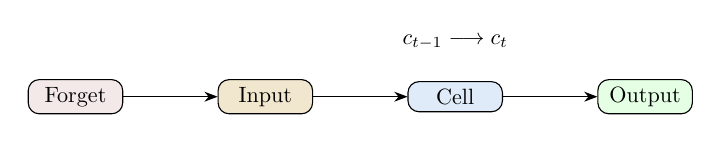
\begin{tikzpicture}[>=Stealth, node distance=1.2cm, scale=0.8, every node/.style={scale=0.8}]
    \node[draw, rounded corners, fill=UoERed!10, minimum width=1.5cm] (forget) {Forget};
    \node[draw, rounded corners, fill=UoEGold!20, minimum width=1.5cm, right=of forget] (input) {Input};
    \node[draw, rounded corners, fill=UoEBlue!15, minimum width=1.5cm, right=of input] (cell) {Cell};
    \node[draw, rounded corners, fill=green!10, minimum width=1.5cm, right=of cell] (output) {Output};
    \draw[->] (forget) -- (input);
    \draw[->] (input) -- (cell);
    \draw[->] (cell) -- (output);
    \node[above=0.3cm of cell] {$c_{t-1} \longrightarrow c_t$};
\end{tikzpicture}
\end{frame}

\section{Practical Considerations}

\begin{frame}{When to Use Neural Networks?}
\begin{center}
\begin{tabular}{lcc}
\toprule
\textbf{Method} & \textbf{Strengths} & \textbf{Weaknesses} \\
\midrule
ARMA & Interpretable, theory & Linear \\
Exponential Smoothing & Trend + season & Univariate \\
VAR & Multivariate dynamics & Many parameters \\
Ridge/Lasso & Many predictors & Still linear \\
Random Forest & Nonlinear & No uncertainty \\
\alert{Neural Networks} & \alert{Universal approx.} & \alert{Data-hungry, opaque} \\
\bottomrule
\end{tabular}
\end{center}

\vspace{0.5em}
\textbf{Rule of thumb:} start simple (ARMA, ETS). Add complexity only if justified by the data.
\end{frame}

\begin{frame}{Course Summary}
\begin{enumerate}
    \item Time series \textbf{components and stationarity}
    \item \textbf{Probability} and estimation
    \item \textbf{ARMA}: the linear workhorse
    \item \textbf{Forecasting}: estimation, selection, evaluation
    \item \textbf{Exponential smoothing}: trend and season
    \item \textbf{VAR}: multivariate dynamics
    \item \textbf{State space}: unobserved components
    \item \textbf{Dynamic factors}: large panels
    \item \textbf{Machine learning}: regularisation, trees
    \item \textbf{Neural networks}: nonlinear frontiers
\end{enumerate}
\end{frame}


\end{document}
